% Set the overall layout of the tree
\tikzstyle{level 1}=[level distance=2.5cm,sibling distance=2cm]
\tikzstyle{level 2}=[level distance=2.5cm,sibling distance=2cm]

% Define styles for bags and leafs
\tikzstyle{bag}=[rectangle,draw=black,text width=4em,text centered]
\tikzstyle{end}=[circle,draw=black,minimum width=3pt,fill,inner sep=0pt]

\begin{figure}
	\centering
	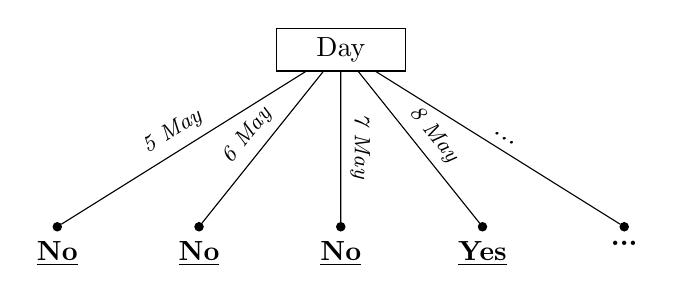
\begin{tikzpicture}[
		scale=0.9,
		sloped
	]
		\node[bag]{\highlighttt{Day}}
    		child{
     		   	node[end,label=below:{\textbf{\underline{No}}}]{}      
     	       	edge from parent 
      		      	node[above]{\textit{\footnotesize 5 May}}
    		}
		child{
        		node[end,label=below:{\textbf{\underline{No}}}]{}      
            		edge from parent 
            		node[above]{\textit{\footnotesize 6 May}}
    		}
    		child{
        		node[end,label=below:{\textbf{\underline{No}}}]{}      
            		edge from parent 
            		node[above]{\textit{\footnotesize 7 May}}
    		}
		child{
        		node[end,label=below:{\textbf{\underline{Yes}}}]{}      
            		edge from parent 
            		node[above]{\textit{\footnotesize 8 May}}
    		}
    		child{
        		node[end,label=below:{\textbf{...}}]{}      
            		edge from parent 
            		node[above]{\textit{...}}
    		};
	\end{tikzpicture}
\end{figure}